\documentclass{article}
\usepackage[UTF8]{ctex} 
\usepackage{amsmath}
\usepackage{bm}
\usepackage{amssymb}
\usepackage{geometry}
\usepackage{graphicx}
\usepackage{listings}
\usepackage{tikz}
\usepackage{amsthm}
\usetikzlibrary{shapes.multipart}
\usetikzlibrary{arrows.meta, positioning, shapes.geometric}
\usetikzlibrary{decorations.pathreplacing, fit}
\geometry{a4paper, margin=1.5cm}

\title{图(2)}
\author{Tan Yiqing}
\date{\today}

\begin{document}
\maketitle
    
    \begin{figure}[h]
        \centering
        \includegraphics[width=0.5\textwidth]{D:/program/data_construction/firefly/20250909224712_149_13.jpg}
    \end{figure}

\section{图的存储结构(续)}
\subsection{邻接表}
\indent 邻接矩阵是存在缺点的,当图比较稀疏时,邻接矩阵中大部分元素为0,造成存储空间的浪费。为了解决这个问题,可以采用邻接表来存储图。\\
\indent 邻接矩阵的时间空间复杂度为$O(V^2)$,而邻接表的时间空间复杂度为$O(V+E)$,其中$V$为顶点数,$E$为边数。\\
\subsubsection{基本思想}
\indent 对于图的每个顶点$v_i$,将所有邻接于$v_i$的顶点链成一个单链表,
称为顶点$v_i$的\pmb{边表}(对于有向图则称为出边表),所有边表的头指针和存储顶点信息的一维数组构成了\pmb{顶点表}。
即如下表:

\begin{figure}[h]
    \centering
    \begin{tikzpicture}[
        cell/.style={
            draw,
            minimum width=2.1cm,
            minimum height=1.2cm,
            font=\small,
            align=center
        }
    ]
        % 顶点表(左右两个框)
        \node[cell] (vleft) {vertex};
        \node[cell, right=0pt of vleft] (vright) {firstedge};
        \node[fit=(vleft)(vright), inner sep=0pt] (vtpair) {};
        \node[below=3mm of vtpair, font=\small] {顶点表};

        % 边表(左右两个框)
        \node[cell, right=3.2cm of vright] (eleft) {adjvex};
        \node[cell, right=0pt of eleft] (eright) {next};
        \node[fit=(eleft)(eright), inner sep=0pt] (etpair) {};
        \node[below=3mm of etpair, font=\small] {边表};
    \end{tikzpicture}
\end{figure}

vertex:数据域,存放顶点信息。           
firstedge:指针域,指向边表中第一个结点。 
adjvex:邻接点域,边的终点在顶点表中的下标。
next:指针域,指向边表中的下一个结点。 

\subsubsection{无向图的邻接表}
\begin{enumerate}
    \item 求顶点 i 的度: 顶点i的边表中结点的个数。
    \item 判断顶点 i 和顶点 j 之间是否存在边:测试顶点 i 的边表中是否存在终点为 j 的结点。
\end{enumerate}

\subsubsection{有向图的邻接表}
\begin{enumerate}
    \item 顶点 i 的出度: 顶点 i 的出边表中结点的个数。
    \item 顶点 i 的入度: 各顶点的出边表中以顶点 i 为终点的结点个数。
    \item 顶点 i 的所有邻接点: 遍历顶点 i 的边表,该边表中的所有终点都是顶点 i 的邻接点。
\end{enumerate}

\subsubsection{网图的邻接表}
\indent 存储的时候带上权值即可。


\subsection{十字链表}
\begin{figure}[h]
    \centering
    \begin{tikzpicture}[
        cell/.style={
            draw,
            minimum width=2.0cm,
            minimum height=1.2cm,
            font=\small,
            align=center
        }
    ]
        % 顶点表(三个框,左右排)
        \node[cell] (vx1) {vertex};
        \node[cell, right=0pt of vx1] (vx2) {firstin};
        \node[cell, right=0pt of vx2] (vx3) {firstout};
        \node[fit=(vx1)(vx3), inner sep=0pt] (vxtuple) {};
        \node[below=3mm of vxtuple, font=\small] {顶点表(十字链表)};

        % 边表(四个框,左右排)
        \node[cell, right=2.2cm of vx3] (ex1) {tailvex};
        \node[cell, right=0pt of ex1] (ex2) {headvex};
        \node[cell, right=0pt of ex2] (ex3) {headlink};
        \node[cell, right=0pt of ex3] (ex4) {taillink};
        \node[fit=(ex1)(ex4), inner sep=0pt] (extuple) {};
        \node[below=3mm of extuple, font=\small] {边表(十字链表)};
    \end{tikzpicture}
\end{figure}

\indent 十字链表是一种用于表示有向图的数据结构,它结合了邻接表和逆邻接表的特点。每个顶点不仅包含指向其出边的指针,还包含指向其入边的指针,从而实现对有向图的高效存储和操作。\\
    \begin{figure}[h]
        \centering
        \includegraphics[width=0.5\textwidth]{D:/program/data_construction/L6/理论/图2/20251117182616.png}
    \end{figure}

\section{最短路径}
\subsection{基本概念}
\indent 在非网图中,最短路径是指两顶点之间经历的边数最少的路径。 
在网图中,最短路径是指两顶点之间经历的边上权值之和最短的路径。\\
\indent \pmb{问:}给定带权有向图$G(V, E)$和源点(入度为0的点)$v∈V$,求从v到G中其余各顶点的最短路径。


\subsection{Dijkstra算法}
\subsubsection{算法思想}
\indent 这类问题有一个特点,假如$A->V_1->V_2->...->V_k->B$是从A到B的最短路径,那么$A->V_1->V_2->...->V_i$的路径也是A到$V_i$的最短路径。即子问题相似。\\
\indent Dijkstra算法是一种\pmb{贪心算法},其基本思想是:从源点出发,逐步扩展已知最短路径的顶点集合,每次选择当前距离源点最近的顶点,并更新其邻接顶点的距离,直到所有顶点的最短路径都被确定。\\

\subsubsection{算法步骤}
\begin{enumerate}
    \item 初始化数组 $dist[1..n]$、$path[1..n]$ 和集合 $S$。令 $S=\{v\}$、$dist[v]=0$;对每个 $u\neq v$:
    \[
        dist[u]=
        \begin{cases}
            w(v,u), & (v,u)\in E\\
            +\infty, & \text{otherwise}
        \end{cases}
        ,\quad path[u]=
        \begin{cases}
            v, & (v,u)\in E\\
            \varnothing, & \text{otherwise}
        \end{cases}
    \]
    \item while($|S|<n$)循环:
    \begin{enumerate}
        \item 在 $V\!-\!S$ 中从 $dist[]$ 取最小值,其下标为 $k$。
        \item 输出(或记录)当前 $dist[]$ 与 $path[]$ 的状态。
        \item 修改数组:对每条边 $(k,u)$ 且 $u\in V\!-\!S$,若 $dist[k]+w(k,u)<dist[u]$,则
        $dist[u]\leftarrow dist[k]+w(k,u)$,$path[u]\leftarrow k$。
        \item 将顶点 $v_k$ 添加到集合 $S$。
    \end{enumerate}
    \item 终止:返回 $dist[]$ 和 $path[]$;沿 $path$ 可回溯最短路径。\\
\end{enumerate}
注:Dijkstra 要求边权非负。w(v,u) 表示边(v,u)的权值。算法复杂度为$O(n^2)$。


\subsubsection{举例分析}
\indent 给定源点 $v_1$,构造一个带权有向图(5 个顶点,8 条边),顶点按正五边形排布。边与权值如下:
$(v_1,v_2,2)$,$(v_1,v_5,7)$,$(v_1,v_3,10)$,$(v_2,v_3,3)$,$(v_2,v_5,4)$,$(v_5,v_4,2)$,$(v_5,v_3,6)$,$(v_3,v_4,1)$。
\begin{figure}[h]
    \centering
    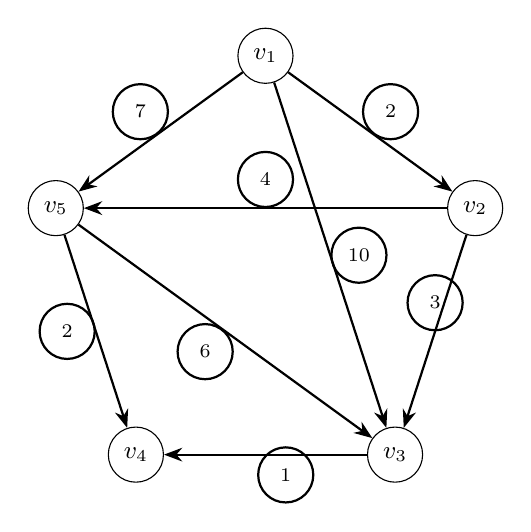
\begin{tikzpicture}[
        >=Stealth,
        every node/.style={circle, draw, minimum size=7mm, font=\small},
        edge/.style={->, thick}
    ]
        % 正五边形坐标(半径2.8)
        \def\r{2.8}
        \path
            (90:\r)   node (v1) {$v_1$}
            (18:\r)   node (v2) {$v_2$}
            (306:\r)  node (v3) {$v_3$}
            (234:\r)  node (v4) {$v_4$}
            (162:\r)  node (v5) {$v_5$};

        % 边与权值
        \draw[edge] (v1) -- (v2) node[midway, above right, font=\scriptsize]{2};
        \draw[edge] (v1) -- (v5) node[midway, above left, font=\scriptsize]{7};
        \draw[edge] (v1) -- (v3) node[midway, right, font=\scriptsize]{10};
        \draw[edge] (v2) -- (v3) node[midway, above, font=\scriptsize]{3};
        \draw[edge] (v2) -- (v5) node[midway, above, font=\scriptsize]{4};
        \draw[edge] (v5) -- (v4) node[midway, left, font=\scriptsize]{2};
        \draw[edge] (v5) -- (v3) node[midway, below left, font=\scriptsize]{6};
        \draw[edge] (v3) -- (v4) node[midway, below right, font=\scriptsize]{1};
    \end{tikzpicture}
\end{figure}

\noindent 距离分析(按“算法步骤”的 2.1→2.2→2.3→2.4 顺序):
\begin{itemize}
    \item 初始化:$S=\{v_1\}$;$dist=\{0,2,10,+\infty,7\}$(对应 $v_1\sim v_5$);$path=\{- ,v_1,v_1,-,v_1\}$。
    \item 第1轮:
    \begin{enumerate}
        \item 选 $k=v_2$(最小 $dist=2$)。
        \item 输出(本轮开始时)$dist=\{0,2,10,+\infty,7\}$,$path=\{- ,v_1,v_1,-,v_1\}$。
        \item 修改:松弛 $v_2\!\to\!v_3:2+3=5<10\Rightarrow dist[v_3]=5,\,path[v_3]=v_2$;松弛 $v_2\!\to\!v_5:2+4=6<7\Rightarrow dist[v_5]=6,\,path[v_5]=v_2$。此后 $dist=\{0,2,5, +\infty,6\}$,$path=\{- ,v_1,v_2,-,v_2\}$。
        \item $S\leftarrow S\cup\{v_2\}$。
    \end{enumerate}
    \item 第2轮:
    \begin{enumerate}
        \item 选 $k=v_3$(最小 $dist=5$)。
        \item 输出:$dist=\{0,2,5,+\infty,6\}$,$path=\{- ,v_1,v_2,-,v_2\}$。
        \item 修改:松弛 $v_3\!\to\!v_4:5+1=6<+\infty\Rightarrow dist[v_4]=6,\,path[v_4]=v_3$。此后 $dist=\{0,2,5,6,6\}$,$path=\{- ,v_1,v_2,v_3,v_2\}$。
        \item $S\leftarrow S\cup\{v_3\}$。
    \end{enumerate}
    \item 第3轮(并列最小 6,取 $v_4$):
    \begin{enumerate}
        \item 选 $k=v_4$。
        \item 输出:$dist=\{0,2,5,6,6\}$,$path=\{- ,v_1,v_2,v_3,v_2\}$。
        \item 修改:$v_4$ 无出边可松弛。
        \item $S\leftarrow S\cup\{v_4\}$。
    \end{enumerate}
    \item 第4轮:
    \begin{enumerate}
        \item 选 $k=v_5$(剩余最小 6)。
        \item 输出:$dist=\{0,2,5,6,6\}$,$path=\{- ,v_1,v_2,v_3,v_2\}$。
        \item 修改:$v_5\!\to\!v_4:6+2=8>6$ 不更新;$v_5\!\to\!v_3:6+6=12>5$ 不更新。
        \item $S\leftarrow S\cup\{v_5\}$,此时 $S=V$,结束。
    \end{enumerate}
\end{itemize}

\noindent 最终 $dist=\{0,2,5,6,6\}$。最短路径:
$v_1\to v_2$;$v_1\to v_2\to v_3$;$v_1\to v_2\to v_3\to v_4$;$v_1\to v_2\to v_5$。

\subsection{Floyd算法}
\subsubsection{算法思想}
\indent \pmb{问题描述:}给定带权有向图$G(V, E)$,对任意顶点$v_i,v_j∈V(i≠j)$,求顶点vi到顶点vj的最短路径。\\
\indent Floyd算法是一种动态规划算法,其基本思想是通过逐步引入中间顶点,更新任意两顶点之间的最短路径,直到考虑所有顶点作为中间顶点为止。\\


\subsection{Floyd算法}
\subsubsection{算法思想}
\indent 基本思想:对任意 $v_i\to v_j$,依次试探以 $v_1,v_2,\dots,v_n$ 作为“中间顶点”的可能性。第 $k$ 次试探时,仅允许中间顶点的编号不大于 $k$,比较两条路径的长度:直接路径 $v_i\to v_j$ 与经由 $v_k$ 的路径 $v_i\to v_k\to v_j$,取较短者作为“当前最优”。经过 $n$ 次比较后,得到 $v_i$ 到 $v_j$ 的最短路径。

\subsubsection{算法步骤}
\begin{enumerate}
    \item 初始化二维矩阵 $dist_{-1}[1..n,1..n]$ 与 $path_{-1}[1..n,1..n]$:
    \[
    dist_{-1}[i,j]=
    \begin{cases}
        0, & i=j\\
        w(i,j), & (i,j)\in E\\
        +\infty, & \text{otherwise}
    \end{cases},\quad
    path_{-1}[i,j]=
    \begin{cases}
        i, & i=j\\
        i\!\to\! j, & (i,j)\in E\\
        \varnothing, & \text{otherwise}
    \end{cases}
    \]
    \item for $k=1$ 到 $n$(第 $k$ 轮):
    \begin{enumerate}
        \item 输出上一轮矩阵 $dist_{k-1}$、$path_{k-1}$。
        \item 对所有 $i,j$,若 $dist_{k-1}[i,k]+dist_{k-1}[k,j]<dist_{k-1}[i,j]$,则
        \[
        dist_k[i,j]\leftarrow dist_{k-1}[i,k]+dist_{k-1}[k,j],\quad
        path_k[i,j]\leftarrow \text{将 }path_{k-1}[i,k]\text{ 与 }path_{k-1}[k,j]\text{ 拼接去重}
        \]
        否则 $dist_k[i,j]\leftarrow dist_{k-1}[i,j]$,$path_k[i,j]\leftarrow path_{k-1}[i,j]$。
        \item 进入下一轮。
    \end{enumerate}
    \item 终止:$dist_{n}$ 与 $path_{n}$ 为所有顶点对的最短距离矩阵与路径矩阵。时间复杂度 $O(n^3)$。可处理负权边但不可存在负环。
\end{enumerate}

\subsubsection{举例分析}
\indent 构造带权有向图(4 个顶点,9 条有向边)。边集与权值:
$(1,2,3)$,$(1,3,10)$,$(1,4,7)$,$(2,3,2)$,$(2,4,6)$,$(3,4,1)$,$(3,1,4)$,$(4,2,1)$,$(4,1,5)$。
\begin{figure}[h]
    \centering
    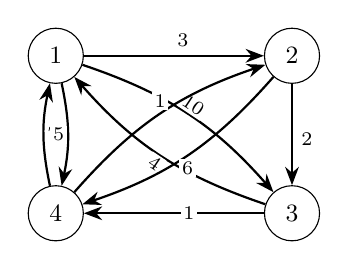
\begin{tikzpicture}[
        >=Stealth, node distance=28mm,
        v/.style={circle, draw, minimum size=7mm, font=\small},
        e/.style={->, thick},
        lab/.style={font=\scriptsize, fill=white, inner sep=1pt}
    ]
        \node[v] (v1) at (0,2) {$1$};
        \node[v] (v2) at (3,2) {$2$};
        \node[v] (v3) at (3,0) {$3$};
        \node[v] (v4) at (0,0) {$4$};

        % 单向边(直线,标签偏移避免重叠)
        \draw[e] (v1)--(v2) node[pos=.55, above=2pt, lab]{3};
        \draw[e] (v2)--(v3) node[pos=.55, right=2pt, lab]{2};
        \draw[e] (v3)--(v4) node[pos=.5, right=2pt, lab]{1};

        % 1 <-> 3 用相反弯曲方向分开
        \draw[e, bend left=15] (v1) to node[pos=.5, above, sloped, lab]{10} (v3);
        \draw[e, bend left=15] (v3) to node[pos=.5, below, sloped, lab]{4} (v1);

        % 1 <-> 4 用相反弯曲方向分开
        \draw[e, bend left=12] (v1) to node[pos=.5, left=2pt, lab]{7} (v4);
        \draw[e, bend left=12] (v4) to node[pos=.5, right=2pt, lab]{5} (v1);

        % 2 <-> 4 用相反弯曲方向分开
        \draw[e, bend left=15] (v2) to node[pos=.5, below=1pt, lab]{6} (v4);
        \draw[e, bend left=15] (v4) to node[pos=.5, above=1pt, lab]{1} (v2);
    \end{tikzpicture}
\end{figure}

\noindent 初始化矩阵($dist_{-1}$ 为邻接矩阵,$path_{-1}$ 为原始路径矩阵):
\[
\scriptsize
dist_{-1}=
\begin{bmatrix}
0&3&10&7\\
\infty&0&2&6\\
4&\infty&0&1\\
5&1&\infty&0
\end{bmatrix},\quad
path_{-1}=
\begin{bmatrix}
1&1\!\to\!2&1\!\to\!3&1\!\to\!4\\
\varnothing&2&2\!\to\!3&2\!\to\!4\\
3\!\to\!1&\varnothing&3&3\!\to\!4\\
4\!\to\!1&4\!\to\!2&\varnothing&4
\end{bmatrix}
\]

\noindent 第1轮(允许中间顶点≤1),得到 $dist_{0}, path_{0}$:
\[
\scriptsize
dist_{0}=
\begin{bmatrix}
0&3&10&7\\
\infty&0&2&6\\
4&7&0&1\\
5&1&15&0
\end{bmatrix},\quad
path_{0}=
\begin{bmatrix}
1&1\!\to\!2&1\!\to\!3&1\!\to\!4\\
\varnothing&2&2\!\to\!3&2\!\to\!4\\
3\!\to\!1&3\!\to\!1\!\to\!2&3&3\!\to\!4\\
4\!\to\!1&4\!\to\!2&4\!\to\!1\!\to\!3&4
\end{bmatrix}
\]

\noindent 第2轮(允许中间顶点≤2),得到 $dist_{1}, path_{1}$:
\[
\scriptsize
dist_{1}=
\begin{bmatrix}
0&3&5&7\\
\infty&0&2&6\\
4&7&0&1\\
5&1&3&0
\end{bmatrix},\quad
path_{1}=
\begin{bmatrix}
1&1\!\to\!2&1\!\to\!2\!\to\!3&1\!\to\!4\\
\varnothing&2&2\!\to\!3&2\!\to\!4\\
3\!\to\!1&3\!\to\!1\!\to\!2&3&3\!\to\!4\\
4\!\to\!1&4\!\to\!2&4\!\to\!2\!\to\!3&4
\end{bmatrix}
\]

\noindent 第3轮(允许中间顶点≤3),得到 $dist_{2}, path_{2}$:
\[
\scriptsize
dist_{2}=
\begin{bmatrix}
0&3&5&6\\
6&0&2&3\\
4&7&0&1\\
5&1&3&0
\end{bmatrix},\quad
path_{2}=
\begin{bmatrix}
1&1\!\to\!2&1\!\to\!2\!\to\!3&1\!\to\!2\!\to\!3\!\to\!4\\
2\!\to\!3\!\to\!1&2&2\!\to\!3&2\!\to\!3\!\to\!4\\
3\!\to\!1&3\!\to\!1\!\to\!2&3&3\!\to\!4\\
4\!\to\!1&4\!\to\!2&4\!\to\!2\!\to\!3&4
\end{bmatrix}
\]

\noindent 第4轮(允许中间顶点≤4),得到最终 $dist_{3}, path_{3}$:
\[
\scriptsize
dist_{3}=
\begin{bmatrix}
0&3&5&6\\
6&0&2&3\\
4&2&0&1\\
5&1&3&0
\end{bmatrix},\quad
path_{3}=
\begin{bmatrix}
1&1\!\to\!2&1\!\to\!2\!\to\!3&1\!\to\!2\!\to\!3\!\to\!4\\
2\!\to\!3\!\to\!1&2&2\!\to\!3&2\!\to\!3\!\to\!4\\
3\!\to\!1&3\!\to\!4\!\to\!2&3&3\!\to\!4\\
4\!\to\!1&4\!\to\!2&4\!\to\!2\!\to\!3&4
\end{bmatrix}
\]

\noindent 由 $dist_{3}$ 可读出任意两点最短距离;由 $path_{3}$ 可直接读出对应最短路径。

\section{最小生成树}
\subsection{基本概念}
\begin{enumerate}
    \item 生成树:n个顶点的连通图G的生成树是包含G中全部顶点的一个极小连通子图。(恰好含有n-1条边的连通图)
    \item 生成森林:在非连通图中,由每个连通分量都可以得到一棵生成树,
    这些连通分量的生成树就组成了一个非连通图的生成森林。

\end{enumerate}

\newtheorem{proposition}{命题}


\begin{proposition}[边数至少为顶点数则必有回路]
在一个 $n$ 个顶点的无向图 $G=(V,E)$ 中,若边数满足 $|E|\ge n$,则 $G$ 中必存在回路。
\end{proposition}

\begin{proof}
采用数学归纳法按顶点数 $n$ 证明。
\textbf{基例}:当 $n\le 3$ 时,命题显然成立。
\textbf{归纳假设}:设对所有顶点数 $<n$ 的无向图命题成立。
\textbf{归纳步}:考虑任意一个顶点数为 $n$ 的无向图 $G$,且 $|E|\ge n$。分两种情形讨论:
\begin{enumerate}
    \item[1)] $G$ 非连通。设其连通分量为 $G_1,\dots,G_m$,对应顶点数与边数分别为 $|V_i|,|E_i|$。若存在某个分量 $G_t$ 使得 $|E_t|\ge |V_t|$,由归纳假设 $G_t$ 中存在回路,从而 $G$ 中存在回路。否则对所有 $i$ 都有 $|E_i|\le |V_i|-1$,则
    \[
        |E|=\sum_{i=1}^m |E_i|\le \sum_{i=1}^m (|V_i|-1)=\Big(\sum_{i=1}^m |V_i|\Big)-m = n-m < n,
    \]
    与 $|E|\ge n$ 矛盾。因此此情形必有回路。
    \item[2)] $G$ 连通。若存在度为 $1$ 的顶点 $w$,令 $e$ 为其唯一邻边,删去 $w$ 与 $e$ 得图 $G'=(V\setminus\{w\},E\setminus\{e\})$。此时 $|V'|=n-1$ 且
    \[
        |E'|=|E|-1 \ge n-1=|V'|,
    \]
    由归纳假设 $G'$ 中存在回路,故 $G$ 中亦存在回路。若 $G$ 中不存在度为 $1$ 的顶点,则每个顶点度数 $\ge 2$。取 $G$ 中一条极长简单路径 $P=v_1v_2\cdots v_k$。由于 $\deg(v_k)\ge 2$,$v_k$ 必与 $P$ 中某个早先顶点 $v_j$($1\le j\le k-2$)相邻,从而形成回路 $v_jv_{j+1}\cdots v_kv_j$。
\end{enumerate}
综上,命题对 $n$ 成立,归纳完毕。
\end{proof}

主要内容见图(3)

\end{document}